The table-robot calibration was done according to the provided protocol \cite{calibrationProtocol}. All the calculations were done in MATLAB \cite{matlab2024b} using the Robotics Systems Toolbox \cite{roboticsToolbox} and the script is included in the appendix. The placement of the world frame can be seen in figure~\ref{fig:worldFrame}. 

\begin{figure}[H]
  \centering
  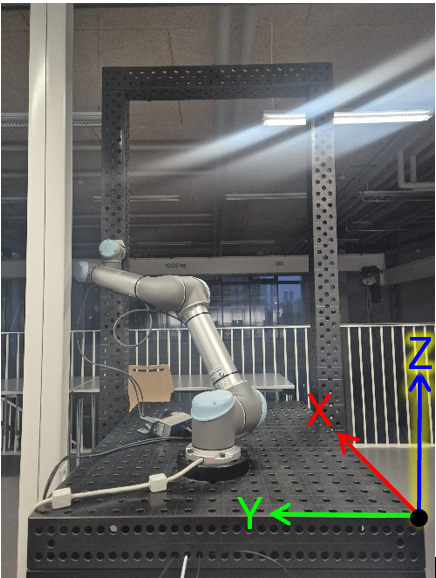
\includegraphics[width=0.5\textwidth]{figures/Worldframe1.png}
  \caption{Placement of the world frame.}
  \label{fig:worldFrame}
\end{figure}

 
Overall, 72 points were measured in both the world frame and robot base frame, and the data is included in the appendix. Of these 72 points, every third point was used for the testing set and the remaining 48 points were used for the training set. The size of the testing set was therefore 24. The calculated world to base transformation is shown below (\ref{eq:world_to_base}). 

\begin{equation}
\label{eq:world_to_base}
\text{world\_to\_base} =
\begin{bmatrix}
0.3841 & -0.9233 & 0.0004 & 0.2743 \\
0.9233 &  0.3841 & -0.0011 & 0.4247 \\
0.0009 &  0.0008 &  1.0000 & 0.0347 \\
0      &  0      &  0      & 1.0000
\end{bmatrix}
\end{equation}

And the corresponding base to world transformation is shown below (\ref{eq:base_to_world}).

\begin{equation}
\label{eq:base_to_world}
\text{base\_to\_world} =
\begin{bmatrix}
0.3841 &  0.9233 &  0.0009 & -0.4975 \\
-0.9233 & 0.3841 &  0.0008 &  0.0902 \\
0.0004 & -0.0011 &  1.0000 & -0.0343 \\
0      &  0      &  0      &  1.0000
\end{bmatrix}
\end{equation}

As the URDF files require the rotational part of the transformation to be provided as “roll pitch yawn” this was also calculated for the world to base transformation. The result is shown below (\ref{eq:rollPitchYawn}).

\begin{equation}
\label{eq:rollPitchYawn}
\text{rollPitchYawn} =
\begin{bmatrix}
0.0008 & -0.0009 & 1.1766
\end{bmatrix}
\end{equation}
 
The base to world transformation was then tested on the 24 points of the testing set to calculate the root mean square error \cite{rmsDeviation} which is shown in the table below (table~\ref{tab:rmsError}). Additionally, the error for each axis in the world frame was also calculated, which is highest in the x-direction and lowest in the z-direction (table~\ref{tab:rmsError}).

\begin{table}[H]
  \centering
  \caption{Overall and per axis root mean square error (mm) \cite{rmsDeviation} for the table-robot calibration.}
  \label{tab:rmsError}
  \begin{tabular}{|l|c|}
    \hline
    Axis in the world frame & Root mean square error (mm) \cite{rmsDeviation} \\ \hline
    Overall & 0.20872 \\
    X-axis  & 0.26483 \\
    Y-axis  & 0.20528 \\
    Z-axis  & 0.13569 \\ \hline
  \end{tabular}
\end{table}

Moreover, a heat map of the x-y plane of the world frame was generated to show local differences for the error. The heat map shows that the local error varies between 0.10 mm and 0.55 mm. The highest local error is for high x-values and low y-values (figure~\ref{fig:heatMap}).

\begin{figure}[H]
  \centering
  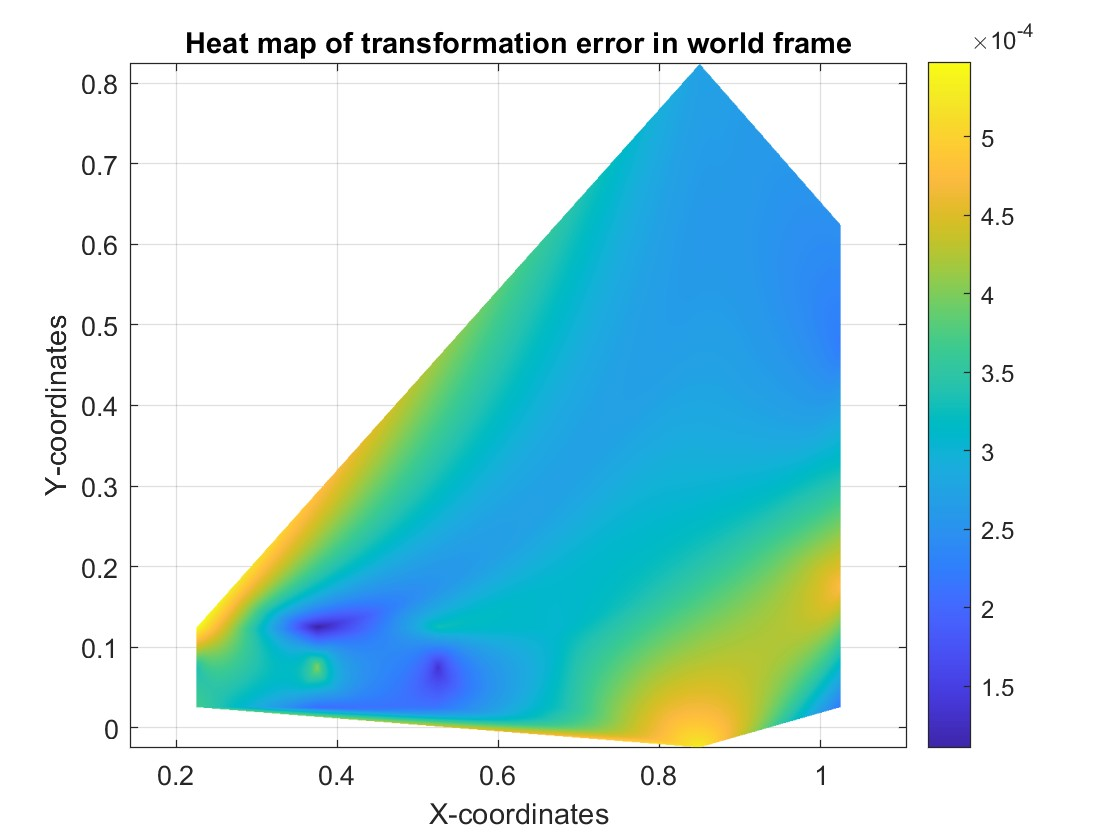
\includegraphics[width=0.7\textwidth]{figures/heatmap_new.jpg}
  \caption{Heatmap of the local calibration error (mm) mapped over the x-y-plane in the world frame.}
  \label{fig:heatMap}
\end{figure}
 
Finally, the errors for different sample sizes of the training set were calculated. The graph shows that the error decreases with increasing sample sizes between sample sizes of 4 and 22 and then stays roughly the same from there until the maximum sample size of 48 (figure~\ref{fig:sampleSizes}).

\begin{figure}[H]
  \centering
  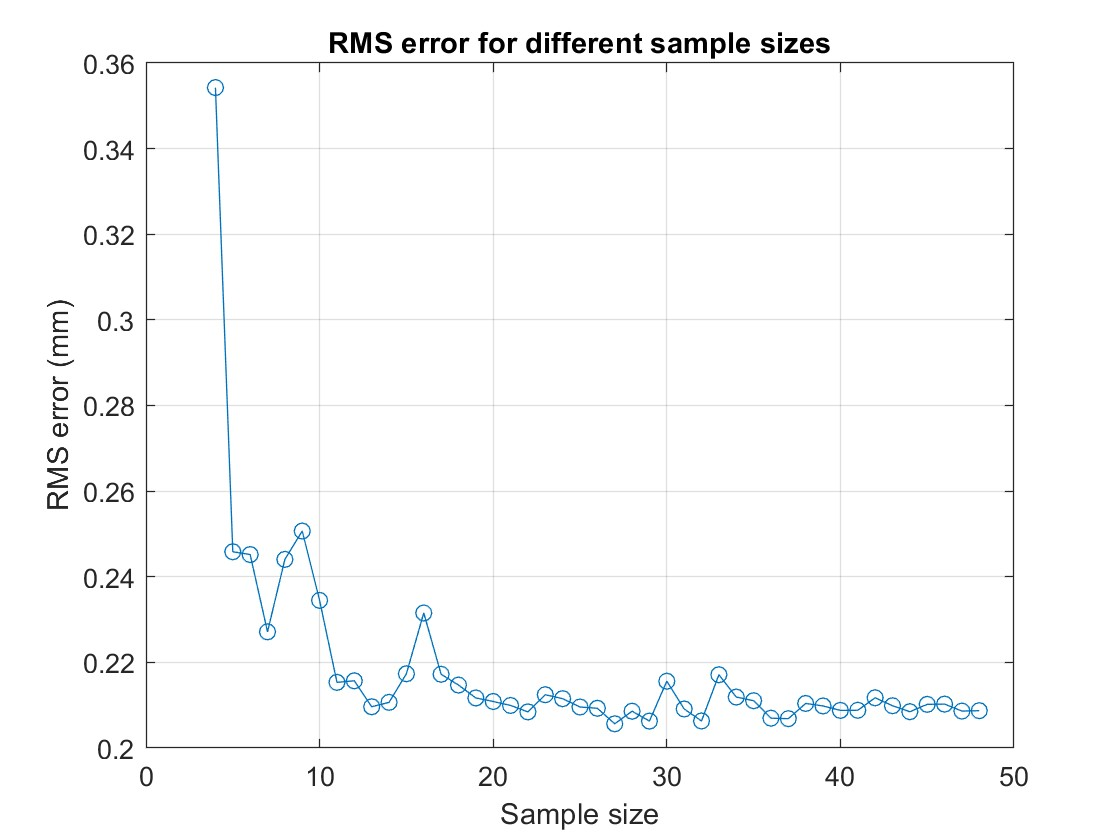
\includegraphics[width=0.7\textwidth]{figures/samplesizes_new.jpg}
  \caption{Root mean square error (mm) for different sample sizes from 4 to 48. The same testing set of 24 points was used on the base to world transformations calculated for each subset of training points.}
  \label{fig:sampleSizes}
\end{figure}
